\documentclass[tikz,border=4pt]{standalone}
\usepackage{tikz}
\usetikzlibrary{positioning, arrows.meta, shapes.geometric}

\definecolor{mutblue}{RGB}{30,90,210}

\begin{document}
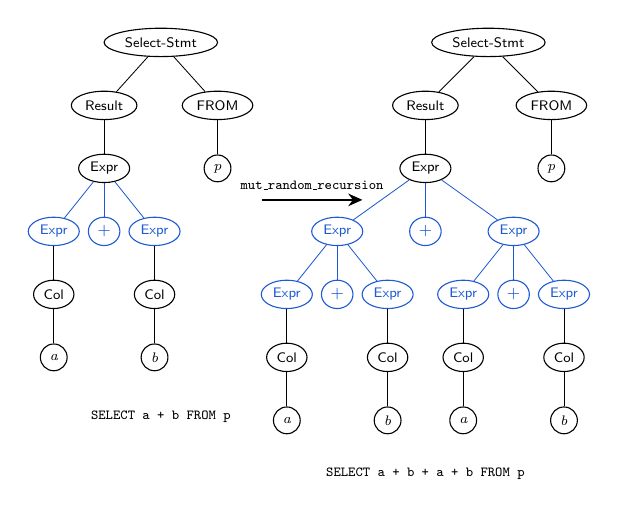
\begin{tikzpicture}[
    x=8mm, y=8mm,
    every node/.style={font=\tiny},
    nt/.style={ellipse, draw=black, line width=0.4pt,
        inner xsep=1.5pt, inner ysep=1pt, font=\tiny\sffamily,
        minimum height=3.6mm},
    op/.style={ellipse, draw=black, line width=0.4pt,
        inner xsep=0.5pt, inner ysep=1pt, font=\tiny\sffamily,
        minimum width=4mm, minimum height=3.6mm},
    lf/.style={circle, draw=black, line width=0.4pt,
        inner sep=0pt, minimum size=3.4mm, font=\tiny\itshape},
    nth/.style={ellipse, draw=mutblue, line width=0.4pt,
        inner xsep=1.5pt, inner ysep=1pt, font=\tiny\sffamily,
        minimum height=3.6mm, text=mutblue},
    oph/.style={ellipse, draw=mutblue, line width=0.4pt,
        inner xsep=0.5pt, inner ysep=1pt, font=\tiny\sffamily,
        minimum width=4mm, minimum height=3.6mm, text=mutblue},
    te/.style={draw=black, line width=0.3pt},
    teh/.style={draw=mutblue, line width=0.3pt},
    mutarrow/.style={-{Stealth[length=1.8mm,width=1.6mm]}, line width=0.6pt},
]

% ====== LEFT: SELECT a + b FROM p ======
\begin{scope}
    \node[nt] (L-root)   at (0,0)    {Select-Stmt};
    \node[nt] (L-result) at (-0.9,-1) {Result};
    \node[nt] (L-from)   at (0.9,-1)  {FROM};

    \node[nt] (L-expr)   at (-0.9,-2) {Expr};
    \node[lf] (L-p)      at (0.9,-2)  {p};

    \node[nth] (L-el)    at (-1.7,-3) {Expr};
    \node[oph] (L-plus)  at (-0.9,-3) {$+$};
    \node[nth] (L-er)    at (-0.1,-3) {Expr};

    \node[nt] (L-cola)  at (-1.7,-4) {Col};
    \node[nt] (L-colb)  at (-0.1,-4) {Col};

    \node[lf] (L-a) at (-1.7,-5) {a};
    \node[lf] (L-b) at (-0.1,-5) {b};

    \foreach \a/\b in {L-root/L-result, L-root/L-from,
        L-result/L-expr, L-from/L-p,
        L-el/L-cola, L-er/L-colb, L-cola/L-a, L-colb/L-b}
        \draw[te] (\a) -- (\b);
    \foreach \a/\b in {L-expr/L-el, L-expr/L-plus, L-expr/L-er}
        \draw[teh] (\a) -- (\b);

    \node[font=\tiny\ttfamily, anchor=north] at (0,-5.7)
        {SELECT a + b FROM p};
\end{scope}

% ====== ARROW ======
\draw[mutarrow] (1.6,-2.5) -- node[above, font=\tiny\ttfamily, align=center]
                                  {mut\_random\_recursion}
                              (3.2,-2.5);

% ====== RIGHT: SELECT a + b + a + b FROM p ======
\begin{scope}[shift={(5.6,0)}]
    \node[nt] (R-root)   at (-0.4,0)  {Select-Stmt};
    \node[nt] (R-result) at (-1.4,-1) {Result};
    \node[nt] (R-from)   at (0.6,-1)  {FROM};

    \node[nt] (R-top)    at (-1.4,-2) {Expr};
    \node[lf] (R-p)      at (0.6,-2)  {p};

    % First split: blue (children of R-top at -1.4, centered)
    \node[nth] (R-left)  at (-2.8,-3) {Expr};
    \node[oph] (R-p0)    at (-1.4,-3) {$+$};
    \node[nth] (R-right) at (0.0,-3)  {Expr};
    % R-top is at -1.4, midpoint of R-left and R-right = (-2.8 + 0.0)/2 = -1.4 ✓

    % Second level splits
    \node[nth] (R-ll)    at (-3.6,-4) {Expr};
    \node[oph] (R-p1)    at (-2.8,-4) {$+$};
    \node[nth] (R-lr)    at (-2.0,-4) {Expr};

    \node[nth] (R-rl)    at (-0.8,-4) {Expr};
    \node[oph] (R-p2)    at ( 0.0,-4) {$+$};
    \node[nth] (R-rr)    at ( 0.8,-4) {Expr};

    \node[nt] (R-c1) at (-3.6,-5) {Col};
    \node[nt] (R-c2) at (-2.0,-5) {Col};
    \node[nt] (R-c3) at (-0.8,-5) {Col};
    \node[nt] (R-c4) at ( 0.8,-5) {Col};

    \node[lf] (R-a1) at (-3.6,-6) {a};
    \node[lf] (R-b1) at (-2.0,-6) {b};
    \node[lf] (R-a2) at (-0.8,-6) {a};
    \node[lf] (R-b2) at ( 0.8,-6) {b};

    \foreach \a/\b in {R-root/R-result, R-root/R-from,
        R-result/R-top, R-from/R-p,
        R-ll/R-c1, R-lr/R-c2, R-rl/R-c3, R-rr/R-c4,
        R-c1/R-a1, R-c2/R-b1, R-c3/R-a2, R-c4/R-b2}
        \draw[te] (\a) -- (\b);
    \foreach \a/\b in {R-top/R-left, R-top/R-p0, R-top/R-right,
        R-left/R-ll, R-left/R-p1, R-left/R-lr,
        R-right/R-rl, R-right/R-p2, R-right/R-rr}
        \draw[teh] (\a) -- (\b);

    \node[font=\tiny\ttfamily, anchor=north] at (-1.4,-6.6)
        {SELECT a + b + a + b FROM p};
\end{scope}

\end{tikzpicture}
\end{document}